\documentclass[aspectratio=169]{beamer}

\usetheme{default}
\usecolortheme{dove}

\setbeamertemplate{navigation symbols}{}
\setbeamertemplate{footline}{%
  \hfill{\large\insertframenumber\,/\,\inserttotalframenumber}\hspace{0.8em}\vspace{0.5em}%
}

\definecolor{popblue}{RGB}{52, 101, 164}
\definecolor{sampred}{RGB}{204, 0, 0}
\definecolor{paramgreen}{RGB}{0, 140, 70}
\definecolor{warnred}{RGB}{180, 40, 40}
\definecolor{orange1}{RGB}{220, 120, 0}
\definecolor{violet1}{RGB}{120, 50, 160}
\definecolor{lightbg}{RGB}{245, 245, 250}

\setbeamercolor{frametitle}{fg=popblue}
\setbeamercolor{title}{fg=popblue}

\usepackage{pgfplots}
\usepackage{tikz}
\usetikzlibrary{shapes, arrows.meta, positioning, calc, decorations.pathreplacing, patterns}
\pgfplotsset{compat=1.18}
\usepackage{amsmath, amssymb}
\usepackage{fontenc}

\title{Lecture 3: Properties of Estimators}
\subtitle{Bias $\cdot$ Variance $\cdot$ MSE $\cdot$ Consistency $\cdot$ Sufficiency $\cdot$ Cram\'er--Rao}
\date{}

\begin{document}

% ============================================================
\begin{frame}
\titlepage
\end{frame}

% ============================================================
\begin{frame}
\frametitle{We use estimators every day. Are they any good?}
\begin{center}
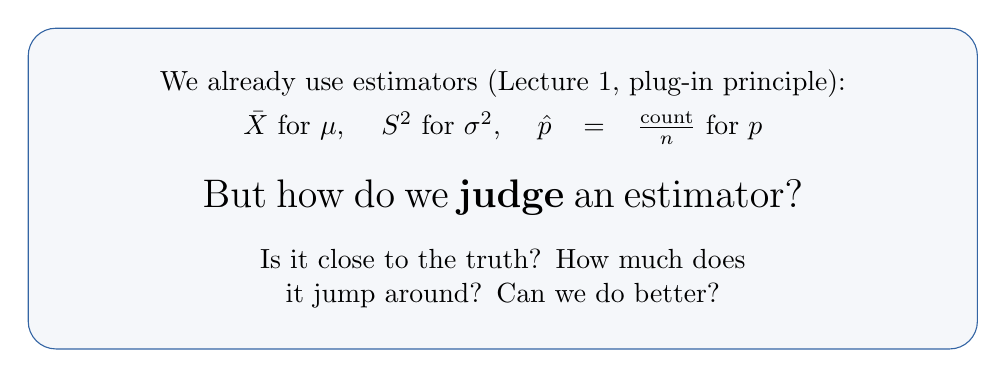
\begin{tikzpicture}
  \node[draw=popblue, fill=popblue!5, rounded corners=10pt, text width=11cm, align=center, inner sep=15pt] {
    We already use estimators (Lecture~1, plug-in principle):\\[4pt]
    $\bar{X}$ for $\mu$, \quad $S^2$ for $\sigma^2$, \quad $\hat{p} = \frac{\text{count}}{n}$ for $p$\\[12pt]
    {\Large But how do we \textbf{judge} an estimator?}\\[10pt]
    Is it close to the truth? How much does it jump around? Can we do better?
  };
\end{tikzpicture}
\end{center}
\end{frame}

% ============================================================
\section{Bias}

\begin{frame}
\frametitle{Bias: Is the Estimator Centered on the Truth?}

$$\text{Bias}(\hat\theta) \;=\; \mathbb{E}[\hat\theta] - \theta$$

\vspace{0.2cm}
\begin{center}
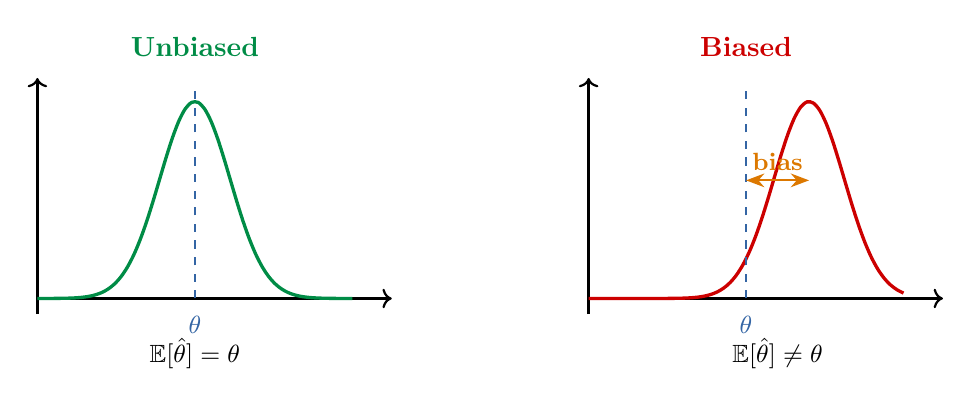
\begin{tikzpicture}
  % Unbiased
  \begin{scope}[xshift=-5cm]
    \node[font=\bfseries, paramgreen] at (2, 3.2) {Unbiased};
    \draw[thick, ->] (0, 0) -- (4.5, 0);
    \draw[thick, ->] (0, -0.2) -- (0, 2.8);
    \draw[very thick, paramgreen, smooth, domain=0:4, samples=50] plot (\x, {2.5*exp(-(\x-2)*(\x-2)/0.4)});
    \draw[dashed, thick, popblue] (2, 0) -- (2, 2.7);
    \node[below, font=\small, popblue] at (2, -0.1) {$\theta$};
    \node[font=\small] at (2, -0.7) {$\mathbb{E}[\hat\theta] = \theta$};
  \end{scope}

  % Biased
  \begin{scope}[xshift=2cm]
    \node[font=\bfseries, sampred] at (2, 3.2) {Biased};
    \draw[thick, ->] (0, 0) -- (4.5, 0);
    \draw[thick, ->] (0, -0.2) -- (0, 2.8);
    \draw[very thick, sampred, smooth, domain=0:4, samples=50] plot (\x, {2.5*exp(-(\x-2.8)*(\x-2.8)/0.4)});
    \draw[dashed, thick, popblue] (2, 0) -- (2, 2.7);
    \node[below, font=\small, popblue] at (2, -0.1) {$\theta$};
    \draw[{Stealth}-{Stealth}, thick, orange1] (2, 1.5) -- (2.8, 1.5);
    \node[above, font=\small\bfseries, orange1] at (2.4, 1.5) {bias};
    \node[font=\small] at (2.4, -0.7) {$\mathbb{E}[\hat\theta] \neq \theta$};
  \end{scope}
\end{tikzpicture}
\end{center}

\vspace{0.1cm}
\begin{center}
\small If $\text{Bias}(\hat\theta) = 0$ for all $\theta$, the estimator is \textbf{unbiased}.
\end{center}
\end{frame}

\begin{frame}
\frametitle{Worked Example: Is $\bar{X}$ Unbiased for $\mu$?}

Let $X_1, \ldots, X_n$ be i.i.d.\ with $\mathbb{E}[X_i] = \mu$. \;Is $\hat\mu = \bar{X} = \frac{1}{n}\sum_{i=1}^n X_i$ unbiased?

\vspace{0.3cm}
\textbf{Step 1:} Compute $\mathbb{E}[\hat\mu]$:
$$\mathbb{E}[\bar{X}] = \mathbb{E}\!\left[\frac{1}{n}\sum_{i=1}^n X_i\right]
= \frac{1}{n}\sum_{i=1}^n \mathbb{E}[X_i]
= \frac{1}{n}\cdot n\mu = \mu$$

\textbf{Step 2:} Check bias:
$$\text{Bias}(\bar{X}) = \mathbb{E}[\bar{X}] - \mu = \mu - \mu = 0 \quad\textcolor{paramgreen}{\checkmark\;\text{Unbiased!}}$$

\vspace{0.2cm}
\begin{center}
\fcolorbox{popblue}{popblue!5}{\parbox{11cm}{\centering\small
  \textbf{Recipe for any estimator:}\\
  (1)~Compute $\mathbb{E}[\hat\theta]$ \;\;$\to$\;\; (2)~Subtract the true $\theta$ \;\;$\to$\;\; (3)~If the result is $0$, it's unbiased.
}}
\end{center}
\end{frame}

\begin{frame}
\frametitle{Worked Example: Why Dividing by $n$ Is Biased}

\small
We want to estimate $\sigma^2$. Natural guess: $\hat\sigma^2_n = \frac{1}{n}\sum_{i=1}^n (X_i - \bar{X})^2$.

\vspace{0.1cm}
\textbf{Key identity} (add and subtract $\mu$):
$$\sum_{i=1}^n (X_i - \bar{X})^2 = \sum_{i=1}^n(X_i - \mu)^2 \;-\; n(\bar{X} - \mu)^2$$

\vspace{-0.2cm}
\textbf{Take expectations:}
\begin{align*}
  \mathbb{E}\!\left[\textstyle\sum(X_i - \mu)^2\right] &= n\sigma^2 &\text{($n$ terms, each } \sigma^2\text{)}\\[-2pt]
  \mathbb{E}\!\left[n(\bar{X} - \mu)^2\right] &= \sigma^2 &\text{(since } \text{Var}(\bar{X}) = \sigma^2/n\text{)}
\end{align*}

\vspace{-0.3cm}
So: $\;\mathbb{E}\!\left[\sum(X_i - \bar{X})^2\right] = n\sigma^2 - \sigma^2 = \textcolor{sampred}{(n-1)\sigma^2}$

\vspace{0.1cm}
\begin{center}
\fcolorbox{sampred}{sampred!5}{\parbox{10cm}{\centering\small
  $\mathbb{E}[\hat\sigma^2_n] = \frac{(n-1)\sigma^2}{n} \neq \sigma^2$ \;\;\textcolor{sampred}{\textbf{Biased!}} It underestimates by $\sigma^2/n$.
}}
\end{center}
\vspace{0.05cm}
\begin{center}
\fcolorbox{paramgreen}{paramgreen!5}{\parbox{10cm}{\centering\small
  \textbf{Bessel's correction:} Divide by $n{-}1$: $\;S^2 = \frac{1}{n-1}\sum(X_i - \bar{X})^2$ \;\;\textcolor{paramgreen}{$\checkmark$ Unbiased}
}}
\end{center}
\end{frame}

\begin{frame}
\frametitle{Bias: Summary}

\renewcommand{\arraystretch}{1.8}
\begin{center}
\begin{tabular}{lcc}
  \textbf{Estimator} & \textbf{Bias} & \textbf{Unbiased?} \\
  \hline
  $\bar{X} = \frac{1}{n}\sum X_i$ \;\text{for}\; $\mu$ &
  $0$ &
  \textcolor{paramgreen}{\textbf{Yes}} \\
  $\hat\sigma^2_n = \frac{1}{n}\sum(X_i-\bar{X})^2$ \;\text{for}\; $\sigma^2$ &
  $-\frac{\sigma^2}{n}$ &
  \textcolor{sampred}{\textbf{No}} \\
  $S^2 = \frac{1}{n-1}\sum(X_i-\bar{X})^2$ \;\text{for}\; $\sigma^2$ &
  $0$ &
  \textcolor{paramgreen}{\textbf{Yes}} \\
  $\hat{p} = \frac{\sum X_i}{n}$ \;\text{for}\; $p$ (Bernoulli) &
  $0$ &
  \textcolor{paramgreen}{\textbf{Yes}} \\
  \hline
\end{tabular}
\end{center}

\vspace{0.3cm}
\begin{center}
\fcolorbox{orange1}{orange1!5}{\parbox{10cm}{\centering\small
  Dividing by $n$ instead of $n{-}1$ \textbf{underestimates} the true variance.\\
  Bessel's correction ($n{-}1$) fixes this. Recall Lecture~2!
}}
\end{center}
\end{frame}

% ============================================================
\section{Variance and MSE}

\begin{frame}
\frametitle{The Dartboard Analogy}
\vspace{-0.2cm}
\begin{center}
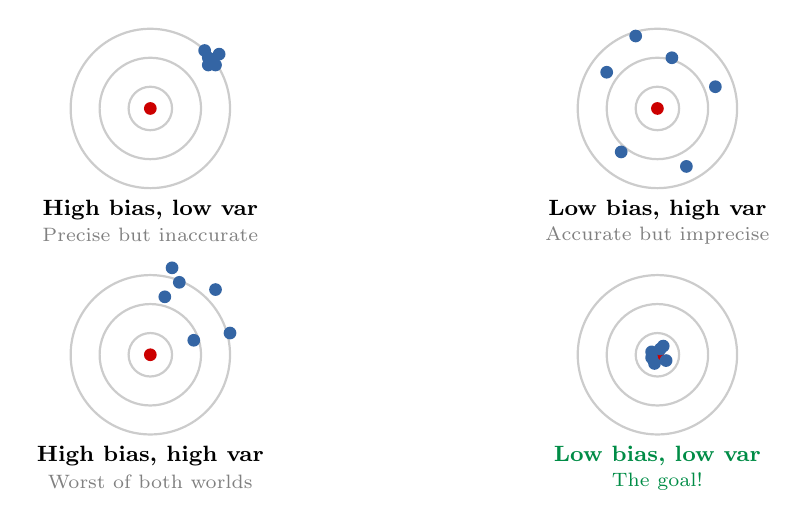
\begin{tikzpicture}[scale=0.92]
  % --- Top-left: High bias, low variance ---
  \begin{scope}[xshift=-3.5cm, yshift=1.2cm]
    \draw[thick, gray!40] (0,0) circle (1.1);
    \draw[thick, gray!40] (0,0) circle (0.7);
    \draw[thick, gray!40] (0,0) circle (0.3);
    \fill[sampred] (0,0) circle (2.5pt);
    \foreach \x/\y in {0.8/0.7, 0.9/0.6, 0.75/0.8, 0.85/0.65, 0.95/0.75, 0.8/0.6} {
      \fill[popblue] (\x, \y) circle (2.5pt);
    }
    \node[font=\footnotesize\bfseries] at (0, -1.4) {High bias, low var};
    \node[font=\scriptsize, gray] at (0, -1.75) {Precise but inaccurate};
  \end{scope}

  % --- Top-right: Low bias, high variance ---
  \begin{scope}[xshift=3.5cm, yshift=1.2cm]
    \draw[thick, gray!40] (0,0) circle (1.1);
    \draw[thick, gray!40] (0,0) circle (0.7);
    \draw[thick, gray!40] (0,0) circle (0.3);
    \fill[sampred] (0,0) circle (2.5pt);
    \foreach \x/\y in {-0.7/0.5, 0.4/-0.8, -0.3/1.0, 0.8/0.3, -0.5/-0.6, 0.2/0.7} {
      \fill[popblue] (\x, \y) circle (2.5pt);
    }
    \node[font=\footnotesize\bfseries] at (0, -1.4) {Low bias, high var};
    \node[font=\scriptsize, gray] at (0, -1.75) {Accurate but imprecise};
  \end{scope}

  % --- Bottom-left: High bias, high variance ---
  \begin{scope}[xshift=-3.5cm, yshift=-2.2cm]
    \draw[thick, gray!40] (0,0) circle (1.1);
    \draw[thick, gray!40] (0,0) circle (0.7);
    \draw[thick, gray!40] (0,0) circle (0.3);
    \fill[sampred] (0,0) circle (2.5pt);
    \foreach \x/\y in {0.4/1.0, 1.1/0.3, 0.2/0.8, 0.9/0.9, 0.6/0.2, 0.3/1.2} {
      \fill[popblue] (\x, \y) circle (2.5pt);
    }
    \node[font=\footnotesize\bfseries] at (0, -1.4) {High bias, high var};
    \node[font=\scriptsize, gray] at (0, -1.75) {Worst of both worlds};
  \end{scope}

  % --- Bottom-right: Low bias, low variance ---
  \begin{scope}[xshift=3.5cm, yshift=-2.2cm]
    \draw[thick, gray!40] (0,0) circle (1.1);
    \draw[thick, gray!40] (0,0) circle (0.7);
    \draw[thick, gray!40] (0,0) circle (0.3);
    \fill[sampred] (0,0) circle (2.5pt);
    \foreach \x/\y in {0.08/0.12, -0.08/-0.04, 0.04/0.08, -0.04/-0.12, 0.12/-0.08, -0.08/0.04} {
      \fill[popblue] (\x, \y) circle (2.5pt);
    }
    \node[font=\footnotesize\bfseries, paramgreen] at (0, -1.4) {Low bias, low var};
    \node[font=\scriptsize, paramgreen] at (0, -1.75) {The goal!};
  \end{scope}
\end{tikzpicture}
\end{center}
\vspace{-0.2cm}
\begin{center}
\small \textcolor{sampred}{Bullseye} = true $\theta$. \;\textcolor{popblue}{Blue dots} = estimates from repeated samples.
\end{center}
\end{frame}

\begin{frame}
\frametitle{Variance of an Estimator}

The \textbf{variance} measures how much $\hat\theta$ wobbles across samples:
$$\text{Var}(\hat\theta) = \mathbb{E}\!\left[(\hat\theta - \mathbb{E}[\hat\theta])^2\right]$$

\vspace{0.3cm}
\begin{center}
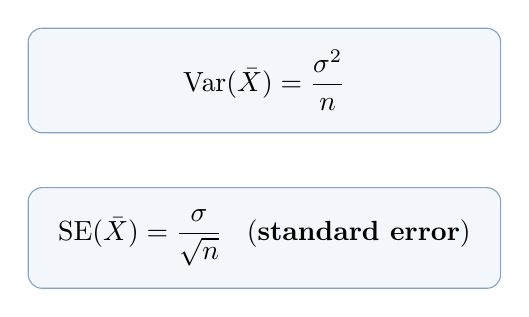
\begin{tikzpicture}[
  ebox/.style={draw=popblue!60, fill=popblue!6, rounded corners=5pt, minimum width=6cm, minimum height=1cm, align=center, font=\normalsize, inner sep=8pt}
]
  \node[ebox] at (0, 1.5) {$\text{Var}(\bar{X}) = \dfrac{\sigma^2}{n}$};
  \node[ebox] at (0, -0.5) {$\text{SE}(\bar{X}) = \dfrac{\sigma}{\sqrt{n}}$ \;\;(\textbf{standard error})};
\end{tikzpicture}
\end{center}

\vspace{0.3cm}
\begin{center}
\small More data $\Rightarrow$ smaller variance $\Rightarrow$ more precise estimate.\\
Variance shrinks at rate $1/n$; standard error at rate $1/\sqrt{n}$.
\end{center}
\end{frame}

\begin{frame}
\frametitle{MSE = Bias$^2$ + Variance: Derivation}

\small
The \textbf{Mean Squared Error}: $\;\text{MSE}(\hat\theta) = \mathbb{E}[(\hat\theta - \theta)^2]$.

\vspace{0.15cm}
\textbf{Trick:} add and subtract $\mathbb{E}[\hat\theta]$:
\begin{align*}
  \hat\theta - \theta
  &= \underbrace{(\hat\theta - \mathbb{E}[\hat\theta])}_{\text{random fluctuation}}
   + \underbrace{(\mathbb{E}[\hat\theta] - \theta)}_{\text{bias (constant)}}
\end{align*}

Square and take expectations:
\begin{align*}
  \mathbb{E}[(\hat\theta - \theta)^2]
  &= \mathbb{E}\!\left[(\hat\theta - \mathbb{E}[\hat\theta])^2\right]
   + 2\underbrace{(\mathbb{E}[\hat\theta] - \theta)}_{\text{constant}} \cdot\underbrace{\mathbb{E}[\hat\theta - \mathbb{E}[\hat\theta]]}_{= \,0}
   + (\mathbb{E}[\hat\theta] - \theta)^2
\end{align*}

\vspace{-0.1cm}
$$\boxed{\text{MSE}(\hat\theta) = \text{Var}(\hat\theta) + \text{Bias}^2(\hat\theta)}$$

\vspace{-0.1cm}
\begin{center}
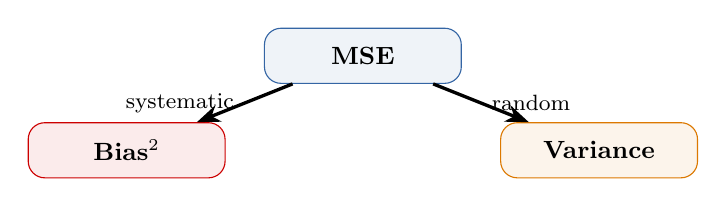
\begin{tikzpicture}
  \node[draw=popblue, fill=popblue!8, rounded corners=6pt, minimum width=2.5cm, minimum height=0.7cm, font=\small] (mse) at (0, 0) {\textbf{MSE}};
  \node[draw=sampred, fill=sampred!8, rounded corners=6pt, minimum width=2.5cm, minimum height=0.7cm, font=\small] (bias) at (-3, -1.2) {\textbf{Bias}$^2$};
  \node[draw=orange1, fill=orange1!8, rounded corners=6pt, minimum width=2.5cm, minimum height=0.7cm, font=\small] (var) at (3, -1.2) {\textbf{Variance}};
  \draw[-{Stealth}, very thick] (mse) -- (bias) node[midway, left, font=\footnotesize] {systematic};
  \draw[-{Stealth}, very thick] (mse) -- (var) node[midway, right, font=\footnotesize] {random};
\end{tikzpicture}
\end{center}
\end{frame}

\begin{frame}
\frametitle{When Biased Beats Unbiased}

\textbf{Example:} Estimating $\sigma^2$ from $X_1,\ldots,X_n \sim N(\mu, \sigma^2)$.

\vspace{0.2cm}
\begin{center}
\renewcommand{\arraystretch}{1.6}
\begin{tabular}{lccc}
  \textbf{Estimator} & \textbf{Bias} & \textbf{Variance} & \textbf{MSE} \\
  \hline
  $S^2 = \frac{1}{n-1}\sum(X_i - \bar{X})^2$ & $0$ & $\frac{2\sigma^4}{n-1}$ & $\frac{2\sigma^4}{n-1}$ \\[6pt]
  $\hat\sigma^2_n = \frac{1}{n}\sum(X_i - \bar{X})^2$ & $-\frac{\sigma^2}{n}$ & $\frac{2(n-1)\sigma^4}{n^2}$ & $\frac{(2n-1)\sigma^4}{n^2}$ \\[6pt]
  \hline
\end{tabular}
\end{center}

\vspace{0.2cm}
\begin{center}
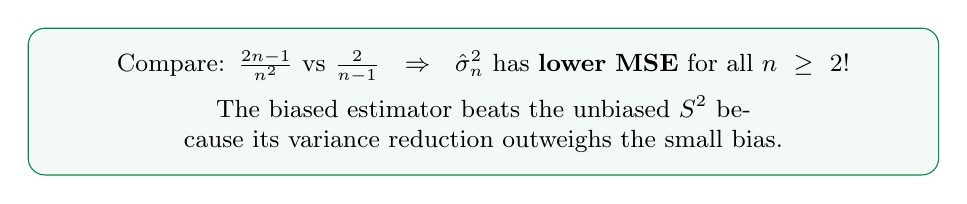
\begin{tikzpicture}
  \node[draw=paramgreen, fill=paramgreen!5, rounded corners=6pt, text width=11cm, align=center, inner sep=8pt, font=\small] {
    Compare: $\frac{2n-1}{n^2}$ vs $\frac{2}{n-1}$ $\;\Rightarrow\;$ $\hat\sigma^2_n$ has \textbf{lower MSE} for all $n \geq 2$!\\[4pt]
    The biased estimator beats the unbiased $S^2$ because its variance reduction outweighs the small bias.
  };
\end{tikzpicture}
\end{center}
\end{frame}

\begin{frame}
\frametitle{MSE Comparison: Visualized}

\small
How do $S^2$ (unbiased, divides by $n{-}1$) and $\hat\sigma^2_n$ (biased, divides by $n$) compare as $n$ grows?

\vspace{0.1cm}
\begin{center}
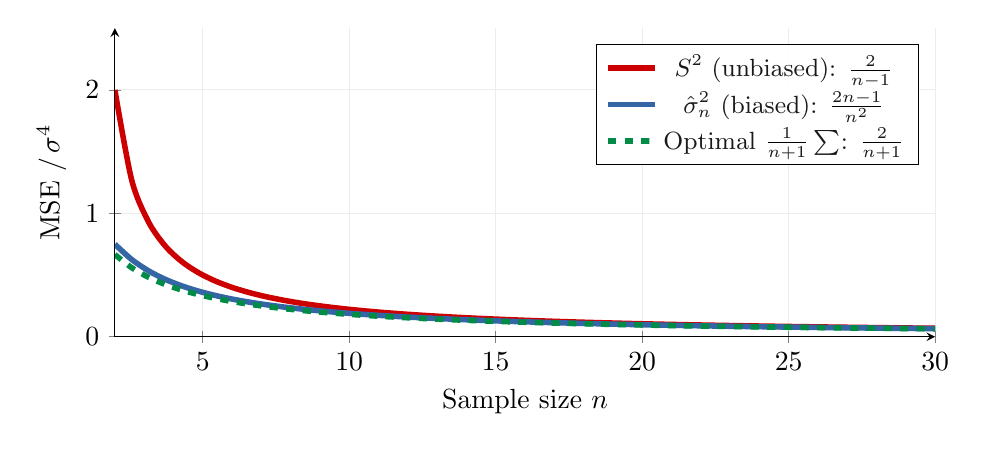
\begin{tikzpicture}
  \begin{axis}[
    width=12cm, height=5.5cm,
    xlabel={Sample size $n$},
    ylabel={MSE $/\, \sigma^4$},
    xmin=2, xmax=30,
    ymin=0, ymax=2.5,
    axis lines=left,
    grid=major, grid style={gray!15},
    every axis plot/.append style={line width=2pt, smooth, samples=50},
    legend style={at={(0.98,0.95)}, anchor=north east, font=\small, fill=white, fill opacity=0.9},
  ]
    % S^2: MSE = 2/(n-1)
    \addplot[sampred, domain=2:30] {2/(x-1)};
    \addlegendentry{$S^2$ (unbiased): $\frac{2}{n-1}$}

    % sigma_hat_n^2: MSE = (2n-1)/n^2
    \addplot[popblue, domain=2:30] {(2*x-1)/(x*x)};
    \addlegendentry{$\hat\sigma^2_n$ (biased): $\frac{2n-1}{n^2}$}

    % Optimal: MSE = 2/(n+1) (divides by n+1)
    \addplot[paramgreen, dashed, domain=2:30] {2/(x+1)};
    \addlegendentry{Optimal $\frac{1}{n+1}\sum$: $\frac{2}{n+1}$}
  \end{axis}
\end{tikzpicture}
\end{center}

\vspace{-0.1cm}
\begin{center}
\small The \textbf{biased} estimator (blue) always beats the unbiased one (red).\\
The optimal divisor is actually $n{+}1$, not $n$ or $n{-}1$ --- even more biased, even lower MSE!
\end{center}
\end{frame}

% ============================================================
\section{Bias-Variance Tradeoff}

\begin{frame}
\frametitle{The Bias-Variance Tradeoff}
\begin{center}
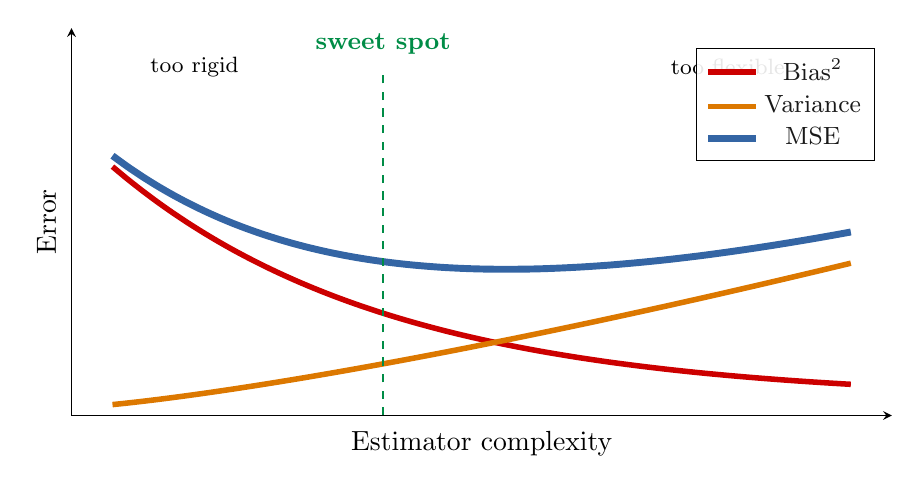
\begin{tikzpicture}
  \begin{axis}[
    width=12cm, height=6.5cm,
    xlabel={Estimator complexity},
    ylabel={Error},
    xmin=0, xmax=10,
    ymin=0, ymax=5,
    xtick=\empty,
    ytick=\empty,
    axis lines=left,
    every axis plot/.append style={line width=2pt, smooth, samples=50},
    legend style={at={(0.98,0.95)}, anchor=north east, font=\small, fill=white, fill opacity=0.9},
  ]
    % Bias^2 (decreasing)
    \addplot[sampred, domain=0.5:9.5] {3.5*exp(-0.3*x) + 0.2};
    \addlegendentry{Bias$^2$}

    % Variance (increasing)
    \addplot[orange1, domain=0.5:9.5] {0.1*x^1.3 + 0.1};
    \addlegendentry{Variance}

    % MSE (U-shaped)
    \addplot[popblue, domain=0.5:9.5, line width=2.5pt] {3.5*exp(-0.3*x) + 0.1*x^1.3 + 0.3};
    \addlegendentry{MSE}

    % Optimal point
    \draw[dashed, thick, paramgreen] (axis cs:3.8, 0) -- (axis cs:3.8, 4.5);
    \node[font=\small\bfseries, paramgreen] at (axis cs:3.8, 4.8) {sweet spot};

    % Annotations
    \node[font=\footnotesize] at (axis cs:1.5, 4.5) {too rigid};
    \node[font=\footnotesize] at (axis cs:8, 4.5) {too flexible};
  \end{axis}
\end{tikzpicture}
\end{center}
\end{frame}

% ============================================================
\section{Consistency}

\begin{frame}
\frametitle{Consistency: Getting It Right Eventually}

An estimator $\hat\theta_n$ is \textbf{consistent} if it converges to the truth as $n \to \infty$:
$$\hat\theta_n \xrightarrow{P} \theta \qquad\text{i.e.,}\quad \Pr\!\left(|\hat\theta_n - \theta| > \varepsilon\right) \to 0 \;\;\text{for all } \varepsilon > 0$$

\vspace{0.3cm}
\begin{center}
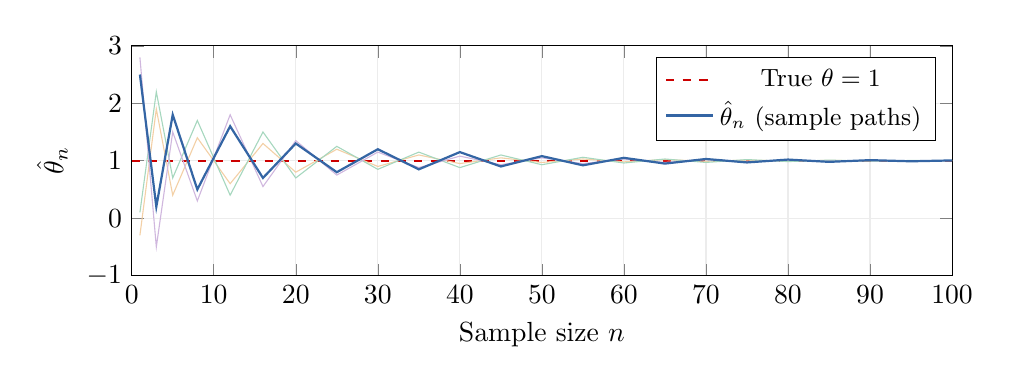
\begin{tikzpicture}
  \begin{axis}[
    width=12cm, height=4.5cm,
    xlabel={Sample size $n$},
    ylabel={$\hat\theta_n$},
    xmin=0, xmax=100,
    ymin=-1, ymax=3,
    grid=major, grid style={gray!15},
    legend style={at={(0.98,0.95)}, anchor=north east, font=\small},
  ]
    % True value
    \addplot[dashed, thick, sampred, domain=0:100] {1};
    \addlegendentry{True $\theta = 1$}

    % Faded sample paths (show many realizations converging)
    \addplot[orange1!35, thin, mark=none, forget plot] coordinates {
      (1, -0.3) (3, 1.9) (5, 0.4) (8, 1.4) (12, 0.6) (16, 1.3)
      (20, 0.8) (25, 1.2) (30, 0.9) (35, 1.1) (40, 0.95)
      (45, 1.05) (50, 0.97) (55, 1.03) (60, 0.98) (65, 1.02)
      (70, 0.99) (75, 1.01) (80, 0.995) (85, 1.005) (90, 0.998) (95, 1.002) (100, 1.001)
    };
    \addplot[paramgreen!35, thin, mark=none, forget plot] coordinates {
      (1, 0.1) (3, 2.2) (5, 0.7) (8, 1.7) (12, 0.4) (16, 1.5)
      (20, 0.7) (25, 1.25) (30, 0.85) (35, 1.15) (40, 0.88)
      (45, 1.1) (50, 0.93) (55, 1.06) (60, 0.96) (65, 1.03)
      (70, 0.97) (75, 1.02) (80, 0.985) (85, 1.01) (90, 0.993) (95, 1.004) (100, 0.998)
    };
    \addplot[violet1!35, thin, mark=none, forget plot] coordinates {
      (1, 2.8) (3, -0.5) (5, 1.5) (8, 0.3) (12, 1.8) (16, 0.55)
      (20, 1.35) (25, 0.75) (30, 1.15) (35, 0.88) (40, 1.08)
      (45, 0.93) (50, 1.05) (55, 0.95) (60, 1.03) (65, 0.97)
      (70, 1.02) (75, 0.98) (80, 1.01) (85, 0.99) (90, 1.005) (95, 0.997) (100, 1.002)
    };

    % Main sample path (emphasized)
    \addplot[popblue, thick, mark=none] coordinates {
      (1, 2.5) (3, 0.2) (5, 1.8) (8, 0.5) (12, 1.6) (16, 0.7)
      (20, 1.3) (25, 0.8) (30, 1.2) (35, 0.85) (40, 1.15)
      (45, 0.9) (50, 1.08) (55, 0.92) (60, 1.05) (65, 0.95)
      (70, 1.03) (75, 0.97) (80, 1.02) (85, 0.98) (90, 1.01) (95, 0.99) (100, 1.005)
    };
    \addlegendentry{$\hat\theta_n$ (sample paths)}
  \end{axis}
\end{tikzpicture}
\end{center}
\end{frame}

\begin{frame}
\frametitle{Sufficient Conditions for Consistency}
\begin{center}
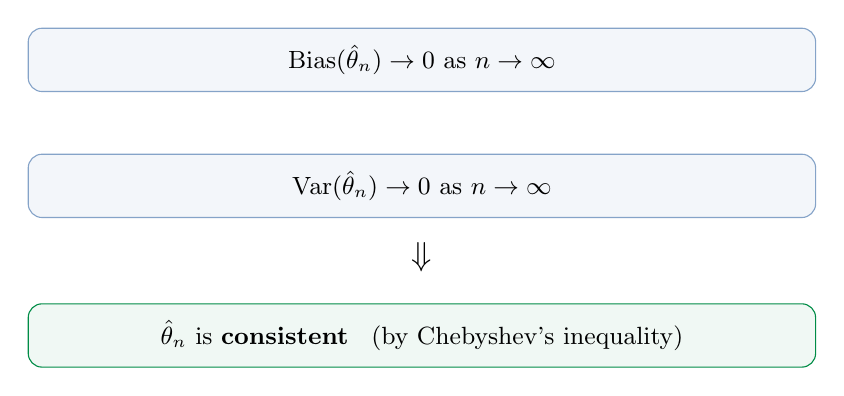
\begin{tikzpicture}[
  sbox/.style={draw=popblue!60, fill=popblue!6, rounded corners=5pt, minimum width=10cm, minimum height=0.8cm, align=center, font=\small, inner sep=6pt}
]
  \node[sbox] at (0, 1.6) {$\text{Bias}(\hat\theta_n) \to 0$ as $n \to \infty$};
  \node[sbox] at (0, 0) {$\text{Var}(\hat\theta_n) \to 0$ as $n \to \infty$};

  \node[font=\large] at (0, -0.9) {$\Downarrow$};

  \node[draw=paramgreen, fill=paramgreen!6, rounded corners=5pt, minimum width=10cm, minimum height=0.8cm, align=center, font=\small, inner sep=6pt]
    at (0, -1.9) {$\hat\theta_n$ is \textbf{consistent} \;\;(by Chebyshev's inequality)};
\end{tikzpicture}
\end{center}

\vspace{0.1cm}
\begin{itemize}\setlength{\itemsep}{2pt}
  \small
  \item The \textbf{sample mean} $\bar{X}_n$ is consistent for $\mu$ (by the Law of Large Numbers)
  \item The \textbf{sample variance} $S^2_n$ is consistent for $\sigma^2$
  \item \textbf{Unbiased + vanishing variance} $\Rightarrow$ consistent. But consistency does \emph{not} require unbiasedness!
\end{itemize}
\end{frame}

% ============================================================
\section{Sufficiency}

\begin{frame}
\frametitle{Sufficiency: Can We Compress the Data?}

\small
We have $n$ data points. Do we really need \textbf{all} of them to estimate $\theta$?

\vspace{0.2cm}
\textbf{Example:} $X_1, \ldots, X_n \sim \text{Bern}(p)$. To estimate $p$:
\begin{itemize}\setlength{\itemsep}{2pt}
  \item We only need $T = \sum X_i$ (total number of successes)
  \item The specific order (HHTHT vs THHTH) tells us nothing more about $p$
\end{itemize}

\vspace{0.2cm}
\begin{center}
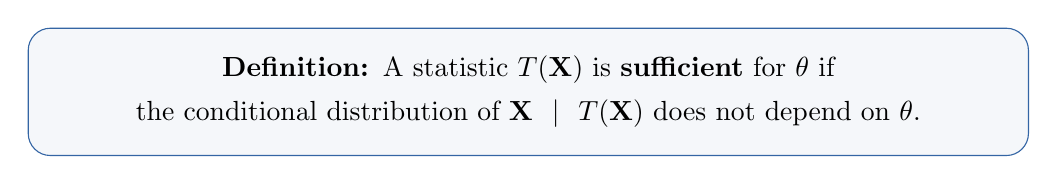
\begin{tikzpicture}
  \node[draw=popblue, fill=popblue!5, rounded corners=8pt, text width=12cm, align=center, inner sep=10pt] {
    \textbf{Definition:} A statistic $T(\mathbf{X})$ is \textbf{sufficient} for $\theta$ if\\[4pt]
    the conditional distribution of $\mathbf{X} \mid T(\mathbf{X})$ does not depend on $\theta$.
  };
\end{tikzpicture}
\end{center}

\vspace{0.2cm}
\begin{center}
\small\textbf{Intuition:} Once you know $T$, the remaining randomness in the data is just noise ---\\
it carries \textbf{no information} about $\theta$. \;$T$ is a ``lossless summary.''
\end{center}
\end{frame}

\begin{frame}
\frametitle{Sufficiency as Data Compression}

\begin{center}
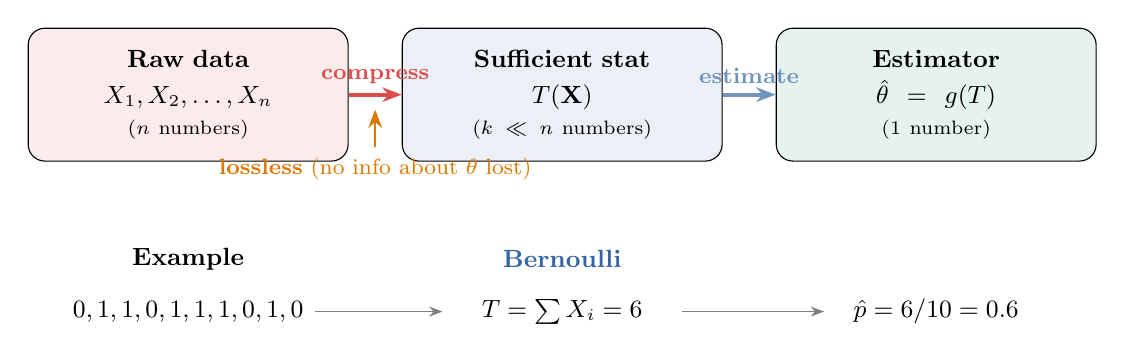
\begin{tikzpicture}[scale=0.95,
  box/.style={draw, rounded corners=6pt, minimum height=1.2cm, align=center, inner sep=8pt, font=\small},
  arrow/.style={-{Stealth[length=7pt]}, line width=1.5pt}
]
  % Raw data
  \node[box, fill=sampred!8, text width=3.5cm] (raw) at (-5, 0) {
    \textbf{Raw data}\\[2pt]
    $X_1, X_2, \ldots, X_n$\\
    {\scriptsize ($n$ numbers)}
  };

  % Sufficient statistic
  \node[box, fill=popblue!10, text width=3.5cm] (suff) at (0, 0) {
    \textbf{Sufficient stat}\\[2pt]
    $T(\mathbf{X})$\\
    {\scriptsize ($k \ll n$ numbers)}
  };

  % Estimator
  \node[box, fill=paramgreen!10, text width=3.5cm] (est) at (5, 0) {
    \textbf{Estimator}\\[2pt]
    $\hat\theta = g(T)$\\
    {\scriptsize (1 number)}
  };

  \draw[arrow, sampred!70] (raw) -- (suff) node[midway, above, font=\footnotesize\bfseries] {compress};
  \draw[arrow, popblue!70] (suff) -- (est) node[midway, above, font=\footnotesize\bfseries] {estimate};

  % Lossless label
  \node[font=\footnotesize, orange1] at (-2.5, -1.0) {\textbf{lossless} (no info about $\theta$ lost)};
  \draw[-{Stealth}, orange1, thick] (-2.5, -0.7) -- (-2.5, -0.2);

  % Examples below
  \node[font=\small\bfseries] at (-5, -2.2) {Example};
  \node[font=\small] at (-5, -2.9) {$0,1,1,0,1,1,1,0,1,0$};

  \node[font=\small\bfseries, popblue] at (0, -2.2) {Bernoulli};
  \node[font=\small] at (0, -2.9) {$T = \sum X_i = 6$};

  \node[font=\small\bfseries, paramgreen] at (5, -2.2) {};
  \node[font=\small] at (5, -2.9) {$\hat{p} = 6/10 = 0.6$};

  % Arrows for example
  \draw[-{Stealth}, gray, thin] (-3.3, -2.9) -- (-1.6, -2.9);
  \draw[-{Stealth}, gray, thin] (1.6, -2.9) -- (3.5, -2.9);
\end{tikzpicture}
\end{center}

\vspace{0.1cm}
\begin{center}
\small The order $(0,1,1,0,1,\ldots)$ doesn't matter for estimating $p$ ---
only the \textbf{total count} matters.
\end{center}
\end{frame}

\begin{frame}
\frametitle{How to Check: Fisher--Neyman Factorization}

\small
\textbf{Theorem:} $T(\mathbf{X})$ is sufficient for $\theta$ if and only if:
$$f(\mathbf{x} \mid \theta) = g\!\left(T(\mathbf{x}),\; \theta\right) \cdot h(\mathbf{x})$$
where $g$ depends on the data \textbf{only through $T$}, and $h$ does not depend on $\theta$.

\vspace{0.15cm}
\textbf{Bernoulli worked example:} $X_1, \ldots, X_n \sim \text{Bern}(p)$, let $T = \sum X_i$.
$$f(\mathbf{x} \mid p) = \prod_{i=1}^n p^{x_i}(1-p)^{1-x_i} = \underbrace{p^{\,\sum x_i}(1-p)^{n - \sum x_i}}_{g(T,\; p)} \cdot \underbrace{1\vphantom{p^{\sum}}}_{h(\mathbf{x})}$$

\vspace{0.1cm}
\begin{center}
\renewcommand{\arraystretch}{1.5}
\begin{tabular}{lll}
  \textbf{Model} & \textbf{Sufficient statistic} & \textbf{Intuition} \\
  \hline
  $\text{Bern}(p)$ & $T = \sum X_i$ & 1 number for 1 parameter \\
  $N(\mu, \sigma^2_0)$ \;($\sigma^2_0$ known) & $T = \bar{X}$ & 1 number for 1 parameter \\
  $N(\mu, \sigma^2)$ \;(both unknown) & $T = (\bar{X},\; S^2)$ & 2 numbers for 2 parameters \\
  \hline
\end{tabular}
\end{center}
\end{frame}

\begin{frame}
\frametitle{Minimal Sufficiency and Why It Matters}

\small
The full data $\mathbf{X}$ is always trivially sufficient. But can we compress \textbf{further}?

\vspace{0.05cm}
\begin{center}
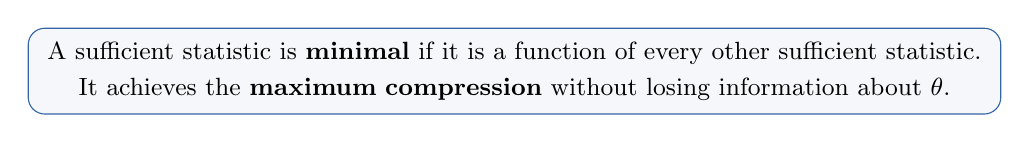
\begin{tikzpicture}
  \node[draw=popblue, fill=popblue!5, rounded corners=6pt, text width=12cm, align=center, inner sep=5pt, font=\small] {
    A sufficient statistic is \textbf{minimal} if it is a function of every other sufficient statistic.\\[2pt]
    It achieves the \textbf{maximum compression} without losing information about $\theta$.
  };
\end{tikzpicture}
\end{center}

\vspace{0.0cm}
\textbf{Example:} For $X_1, \ldots, X_n \sim N(\mu, \sigma^2_0)$ with $\sigma^2_0$ known:

\vspace{-0.15cm}
\begin{itemize}\setlength{\itemsep}{0pt}
  \item $\mathbf{X} = (X_1, \ldots, X_n)$ --- sufficient (trivially), but no compression
  \item $(\bar{X}, S^2)$ --- sufficient, some compression
  \item $\bar{X}$ alone --- sufficient \textbf{and minimal}. Maximum compression!
\end{itemize}

\vspace{-0.05cm}
\begin{center}
\fcolorbox{paramgreen}{paramgreen!5}{\parbox{11cm}{\centering\small
  \textbf{Rao--Blackwell:} Any unbiased $\tilde\theta$ can be improved: $\hat\theta = \mathbb{E}[\tilde\theta \mid T]$ has $\text{Var}(\hat\theta) \leq \text{Var}(\tilde\theta)$.
}}
\end{center}

\vspace{0.0cm}
\small\textbf{In action:} $X_1,\ldots,X_n \sim \text{Bern}(p)$, \;$T = \sum X_i$: \quad
$\underbrace{\tilde{p} = X_1}_{\text{Var} = p(1-p)}$
\;$\xrightarrow{\;\mathbb{E}[\,\cdot\mid T\,]\;}$\;
$\underbrace{\hat{p} = \bar{X}}_{\text{Var} = p(1-p)/n}$
\;\textcolor{paramgreen}{$\boldsymbol{\times n}$ \textbf{better!}}
\end{frame}

\begin{frame}
\frametitle{Finding Minimal Sufficient Statistics}

\small
\textbf{Theorem (Likelihood Ratio Criterion):} $T(\mathbf{X})$ is minimal sufficient iff for all $\mathbf{x}, \mathbf{y}$:

$$T(\mathbf{x}) = T(\mathbf{y}) \quad\Longleftrightarrow\quad \frac{f(\mathbf{x} \mid \theta)}{f(\mathbf{y} \mid \theta)} \;\text{does not depend on}\; \theta$$

\vspace{0.15cm}
\textbf{Bernoulli example:} $X_1, \ldots, X_n \sim \text{Bern}(p)$.

$$\frac{f(\mathbf{x} \mid p)}{f(\mathbf{y} \mid p)}
= \frac{p^{\sum x_i}(1-p)^{n-\sum x_i}}{p^{\sum y_i}(1-p)^{n-\sum y_i}}
= \left(\frac{p}{1-p}\right)^{\!\sum x_i - \sum y_i}$$

Free of $p$ $\;\Longleftrightarrow\;$ $\sum x_i = \sum y_i$.
\;\;So $T = \sum X_i$ is \textbf{minimal sufficient} for $p$. \;\textcolor{paramgreen}{$\checkmark$}

\vspace{0.2cm}
\begin{center}
\fcolorbox{orange1}{orange1!5}{\parbox{11cm}{\centering\small
  \textbf{Recipe:} Write the likelihood ratio $f(\mathbf{x}\mid\theta)/f(\mathbf{y}\mid\theta)$.\\
  Find which function of the data must match for the ratio to lose its $\theta$-dependence.\\
  That function is the minimal sufficient statistic.
}}
\end{center}
\end{frame}

% ============================================================
\section{Exponential Family}

\begin{frame}
\frametitle{The Exponential Family: A Unifying Framework}

\small
All our examples --- Bernoulli, Normal, Poisson, Exponential --- share one structure:

$$\boxed{f(x \mid \theta) = h(x)\;\exp\!\Big(\eta(\theta)\,T(x) - A(\theta)\Big)}$$

\vspace{-0.1cm}
\begin{center}
\renewcommand{\arraystretch}{1.5}
\begin{tabular}{lccc}
  \textbf{Distribution} & \textbf{Natural param}~$\eta(\theta)$ & $T(x)$ & \textbf{Suff.\ stat} ($n$ obs) \\
  \hline
  $\text{Bern}(p)$ & $\log\frac{p}{1-p}$ & $x$ & $\sum X_i$ \\[1pt]
  $N(\mu,\sigma_0^2)$ \;($\sigma_0^2$ known) & $\mu/\sigma_0^2$ & $x$ & $\sum X_i$ \\[1pt]
  $\text{Pois}(\lambda)$ & $\log\lambda$ & $x$ & $\sum X_i$ \\[1pt]
  $\text{Exp}(\lambda)$ & $-\lambda$ & $x$ & $\sum X_i$ \\
  \hline
\end{tabular}
\end{center}

\vspace{0.1cm}
\begin{center}
\fcolorbox{popblue}{popblue!5}{\parbox{11cm}{\centering\small
  \textbf{Pattern:} For single-parameter families, $T(x) = x$. The sufficient statistic\\
  for $n$ observations is always $\sum T(X_i)$ --- straight from the factorization theorem!
}}
\end{center}
\end{frame}

\begin{frame}
\frametitle{Why Exponential Families Are Special}

\small
Nearly every nice property we've discussed is \textbf{automatic} in exponential families:

\vspace{0.05cm}
\begin{center}
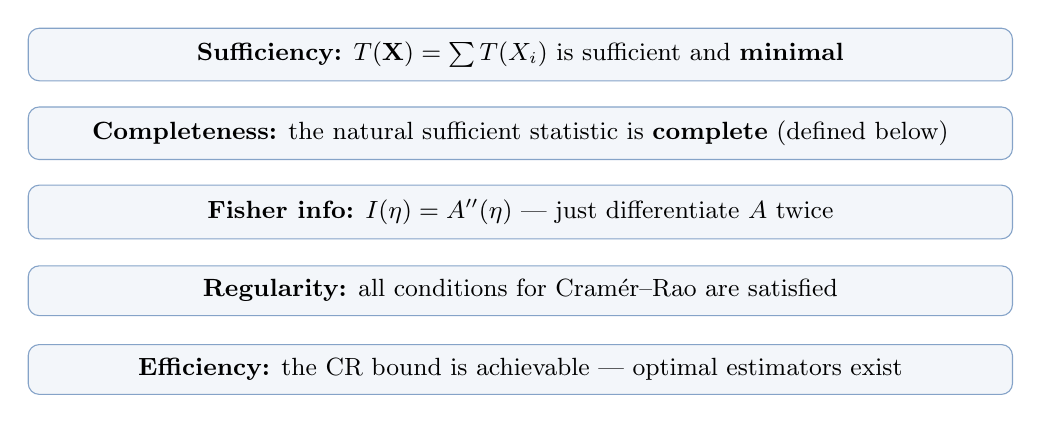
\begin{tikzpicture}[
  pbox/.style={draw=popblue!60, fill=popblue!6, rounded corners=4pt, minimum width=12.5cm, align=left, inner sep=5pt, font=\small}
]
  \node[pbox] at (0, 2.0) {\textbf{Sufficiency:} $T(\mathbf{X}) = \sum T(X_i)$ is sufficient and \textbf{minimal}};
  \node[pbox] at (0, 1.0) {\textbf{Completeness:} the natural sufficient statistic is \textbf{complete} (defined below)};
  \node[pbox] at (0, 0) {\textbf{Fisher info:} $I(\eta) = A''(\eta)$ --- just differentiate $A$ twice};
  \node[pbox] at (0, -1.0) {\textbf{Regularity:} all conditions for Cram\'er--Rao are satisfied};
  \node[pbox] at (0, -2.0) {\textbf{Efficiency:} the CR bound is achievable --- optimal estimators exist};
\end{tikzpicture}
\end{center}

\vspace{0.05cm}
\begin{center}
\fcolorbox{paramgreen}{paramgreen!5}{\parbox{11.5cm}{\centering\small
  \textbf{Completeness:} $T$ is \textbf{complete} if $\mathbb{E}_\theta[g(T)] = 0\;\forall\,\theta \;\Rightarrow\; g(T) = 0$ a.s.\\[1pt]
  \textbf{Lehmann--Scheff\'e:} An unbiased estimator based on a complete sufficient\\[-1pt]
  statistic is the \textbf{unique best} unbiased estimator (UMVUE).
}}
\end{center}
\end{frame}

% ============================================================
\section{Fisher Information and Cram\'er--Rao}

\begin{frame}
\frametitle{Can We Do Better? The Fundamental Question}

\begin{center}
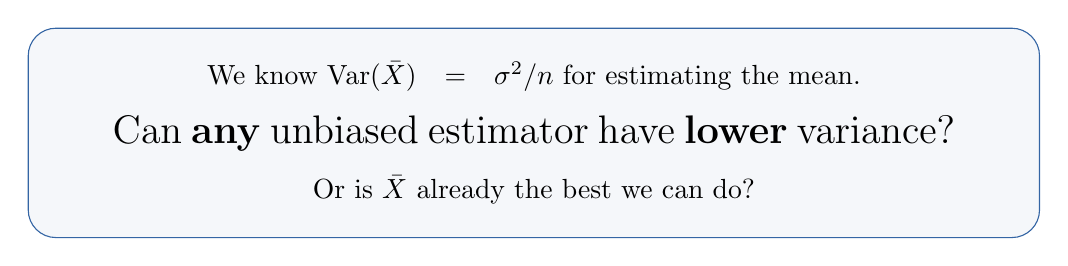
\begin{tikzpicture}
  \node[draw=popblue, fill=popblue!5, rounded corners=10pt, text width=12cm, align=center, inner sep=12pt] {
    We know $\text{Var}(\bar{X}) = \sigma^2/n$ for estimating the mean.\\[8pt]
    {\Large Can \textbf{any} unbiased estimator have \textbf{lower} variance?}\\[8pt]
    Or is $\bar{X}$ already the best we can do?
  };
\end{tikzpicture}
\end{center}

\vspace{0.3cm}
To answer this, we need to measure \textbf{how much information} one observation carries about $\theta$.

\vspace{0.2cm}
\begin{center}
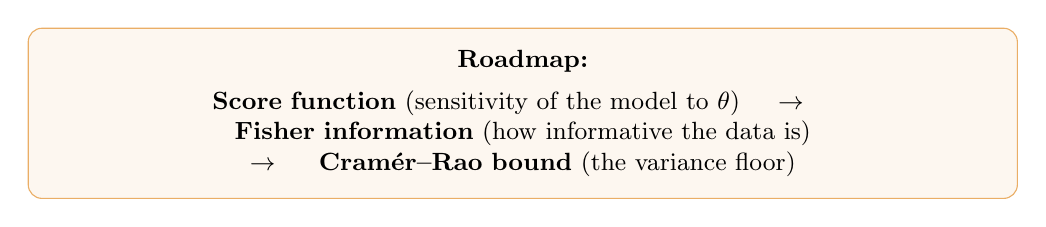
\begin{tikzpicture}
  \node[draw=orange1!60, fill=orange1!6, rounded corners=5pt, text width=12cm, align=center, inner sep=8pt, font=\small] {
    \textbf{Roadmap:}\\[4pt]
    \textbf{Score function} (sensitivity of the model to $\theta$)
    $\;\to\;$ \textbf{Fisher information} (how informative the data is)\\
    $\to\;$ \textbf{Cram\'er--Rao bound} (the variance floor)
  };
\end{tikzpicture}
\end{center}
\end{frame}

\begin{frame}
\frametitle{The Score Function: How Sensitive Is the Model?}

\small
Given a model $f(x \mid \theta)$, the \textbf{score} measures how the log-probability changes with $\theta$:
$$s(\theta) = \frac{\partial}{\partial\theta} \log f(X \mid \theta)$$

\vspace{0.1cm}
\textbf{Concrete example:} $X \sim \text{Bernoulli}(p)$.

\vspace{0.1cm}
$\log f(x \mid p) = x \log p + (1{-}x)\log(1{-}p)$

$$s(p) = \frac{\partial}{\partial p}\left[x \log p + (1{-}x)\log(1{-}p)\right] = \frac{x}{p} - \frac{1-x}{1-p} = \frac{x - p}{p(1-p)}$$

\vspace{0.1cm}
\begin{itemize}\setlength{\itemsep}{3pt}
  \item If we observe $x = 1$ and $p$ is small, the score is \textbf{large positive} $\to$ ``$p$ should be higher''
  \item If we observe $x = 0$ and $p$ is large, the score is \textbf{large negative} $\to$ ``$p$ should be lower''
  \item On average: $\mathbb{E}[s(p)] = 0$ --- the score points in the right direction but \textbf{averages out}
\end{itemize}
\end{frame}

\begin{frame}
\frametitle{Fisher Information: How Informative Is One Observation?}

The score averages to zero, but it \textbf{varies}. More variation $=$ more information:

\vspace{-0.1cm}
$$\boxed{I(\theta) = \text{Var}[s(\theta)] = \mathbb{E}\!\left[\left(\frac{\partial}{\partial\theta}\log f(X \mid \theta)\right)^{\!2}\right]}$$

\vspace{-0.15cm}
\begin{columns}[T]
\begin{column}{0.48\textwidth}
\small
\textbf{Bernoulli example:}
$$I(p) = \frac{\text{Var}(X)}{[p(1{-}p)]^2} = \frac{1}{p(1{-}p)}$$

\vspace{-0.2cm}
\begin{itemize}\setlength{\itemsep}{1pt}
  \scriptsize
  \item $p = 0.5$: $I = 4$ (least informative)
  \item $p = 0.1$: $I = 11.1$ (more informative)
  \item $p = 0.01$: $I = 101$ (most informative)
\end{itemize}

\vspace{0.05cm}
\scriptsize Near $p = 0$ or $1$: each flip tells you a lot.\\At $p = 0.5$: max noise, min information.
\end{column}
\begin{column}{0.50\textwidth}
\begin{center}
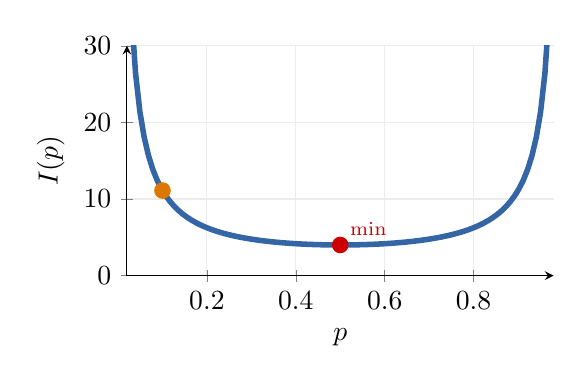
\begin{tikzpicture}
  \begin{axis}[
    width=7cm, height=4.5cm,
    xlabel={$p$},
    ylabel={$I(p)$},
    xmin=0.02, xmax=0.98,
    ymin=0, ymax=30,
    axis lines=left,
    grid=major, grid style={gray!15},
    every axis plot/.append style={line width=2pt, samples=100},
  ]
    \addplot[popblue, domain=0.02:0.98] {1/(x*(1-x))};

    \fill[sampred] (axis cs:0.5, 4) circle (3pt);
    \node[font=\scriptsize, sampred, above right] at (axis cs:0.5, 4) {min};

    \fill[orange1] (axis cs:0.1, 11.11) circle (3pt);
  \end{axis}
\end{tikzpicture}
\end{center}
\end{column}
\end{columns}
\end{frame}

\begin{frame}
\frametitle{Intuition: Sharp vs Flat Log-Likelihood}
\begin{center}
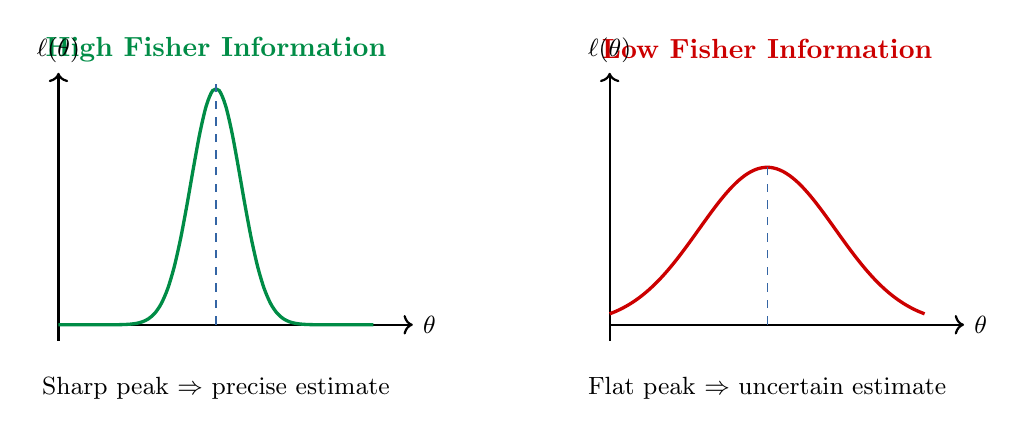
\begin{tikzpicture}
  % High information
  \begin{scope}[xshift=-5cm]
    \node[font=\bfseries, paramgreen] at (2, 3.5) {High Fisher Information};
    \draw[thick, ->] (0, 0) -- (4.5, 0) node[right, font=\small] {$\theta$};
    \draw[thick, ->] (0, -0.2) -- (0, 3.2) node[above, font=\small] {$\ell(\theta)$};
    \draw[very thick, paramgreen, smooth, domain=0:4, samples=50]
      plot (\x, {3*exp(-(\x-2)*(\x-2)/0.2)});
    \draw[dashed, popblue] (2, 0) -- (2, 3.1);
    \node[font=\small] at (2, -0.8) {Sharp peak $\Rightarrow$ precise estimate};
  \end{scope}

  % Low information
  \begin{scope}[xshift=2cm]
    \node[font=\bfseries, sampred] at (2, 3.5) {Low Fisher Information};
    \draw[thick, ->] (0, 0) -- (4.5, 0) node[right, font=\small] {$\theta$};
    \draw[thick, ->] (0, -0.2) -- (0, 3.2) node[above, font=\small] {$\ell(\theta)$};
    \draw[very thick, sampred, smooth, domain=0:4, samples=50]
      plot (\x, {2*exp(-(\x-2)*(\x-2)/1.5)});
    \draw[dashed, popblue] (2, 0) -- (2, 2.1);
    \node[font=\small] at (2, -0.8) {Flat peak $\Rightarrow$ uncertain estimate};
  \end{scope}
\end{tikzpicture}
\end{center}

\vspace{0.2cm}
\begin{center}
\small $I(\theta)$ = \textbf{curvature} of the log-likelihood. Sharp curve $\Rightarrow$ high $I(\theta)$ $\Rightarrow$ data is very informative.\\[4pt]
Equivalently: $I(\theta) = -\mathbb{E}\!\left[\frac{\partial^2}{\partial\theta^2}\log f(X \mid \theta)\right]$ \;(expected negative curvature).
\end{center}
\end{frame}

\begin{frame}
\frametitle{Cram\'er--Rao Lower Bound}

\small
Now we can answer the question: for any \textbf{unbiased} estimator $\hat\theta$ based on $n$ i.i.d.\ observations:

$$\boxed{\text{Var}(\hat\theta) \;\geq\; \frac{1}{n \cdot I(\theta)}}$$

\vspace{0.1cm}
\textbf{Verify for the Bernoulli example:}
\begin{itemize}\setlength{\itemsep}{2pt}
  \item We computed $I(p) = \frac{1}{p(1-p)}$
  \item CR bound: $\text{Var}(\hat{p}) \geq \frac{1}{n \cdot \frac{1}{p(1-p)}} = \frac{p(1-p)}{n}$
  \item Actual variance of $\hat{p} = \bar{X}$: $\;\text{Var}(\hat{p}) = \frac{p(1-p)}{n}$ \;\;\textcolor{paramgreen}{$\checkmark$ Hits the bound exactly!}
\end{itemize}

\vspace{0.1cm}
\begin{center}
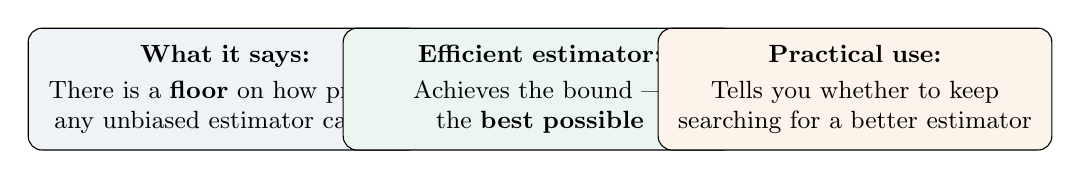
\begin{tikzpicture}[
  cbox/.style={draw, rounded corners=5pt, minimum width=5cm, minimum height=1.5cm, align=center, text width=4.5cm, inner sep=6pt, font=\small}
]
  \node[cbox, fill=popblue!8] at (-4, 0) {
    \textbf{What it says:}\\[2pt]
    There is a \textbf{floor} on how precise any unbiased estimator can be
  };
  \node[cbox, fill=paramgreen!8] at (0, 0) {
    \textbf{Efficient estimator:}\\[2pt]
    Achieves the bound ---\\
    the \textbf{best possible}
  };
  \node[cbox, fill=orange1!8] at (4, 0) {
    \textbf{Practical use:}\\[2pt]
    Tells you whether to keep\\
    searching for a better estimator
  };
\end{tikzpicture}
\end{center}
\end{frame}

\begin{frame}
\frametitle{Regularity Conditions: When Does CR Apply?}

\vspace{-0.2cm}
\small
The Cram\'er--Rao bound requires \textbf{regularity conditions}:

\vspace{0.05cm}
\begin{columns}[T]
\begin{column}{0.50\textwidth}
\footnotesize
\begin{enumerate}\setlength{\itemsep}{0pt}
  \item \textbf{Support} of $f(x \mid \theta)$ doesn't depend on $\theta$
  \item $\theta$ in the \textbf{interior} of the parameter space
  \item Can differentiate under the integral sign
  \item $0 < I(\theta) < \infty$
\end{enumerate}

\vspace{0.1cm}
\small\textbf{Counterexample: $\text{Uniform}(0, \theta)$}
\begin{itemize}\setlength{\itemsep}{0pt}
  \footnotesize
  \item Support $[0, \theta]$ depends on $\theta$!
  \item Suff.\ stat: $X_{(n)} = \max_i X_i$
  \item $\text{Var}(X_{(n)}) \sim 1/n^2$ --- \textbf{faster} than CR
\end{itemize}
\end{column}
\begin{column}{0.48\textwidth}
\vspace{-0.1cm}
\begin{center}
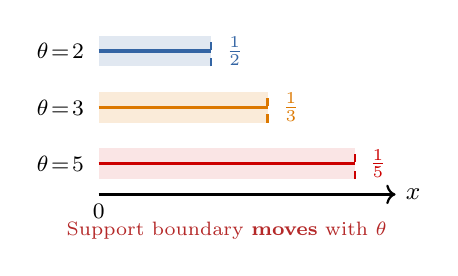
\begin{tikzpicture}[scale=0.65]
  % theta = 2
  \fill[popblue!15] (0, 2.2) rectangle (2.2, 2.8);
  \draw[very thick, popblue] (0, 2.5) -- (2.2, 2.5);
  \draw[thick, popblue, dashed] (2.2, 2.2) -- (2.2, 2.8);
  \node[left, font=\footnotesize] at (-0.1, 2.5) {$\theta\!=\!2$};
  \node[right, font=\footnotesize, popblue] at (2.3, 2.5) {$\frac{1}{2}$};

  % theta = 3
  \fill[orange1!15] (0, 1.1) rectangle (3.3, 1.7);
  \draw[very thick, orange1] (0, 1.4) -- (3.3, 1.4);
  \draw[thick, orange1, dashed] (3.3, 1.1) -- (3.3, 1.7);
  \node[left, font=\footnotesize] at (-0.1, 1.4) {$\theta\!=\!3$};
  \node[right, font=\footnotesize, orange1] at (3.4, 1.4) {$\frac{1}{3}$};

  % theta = 5
  \fill[sampred!10] (0, 0) rectangle (5.0, 0.6);
  \draw[very thick, sampred] (0, 0.3) -- (5.0, 0.3);
  \draw[thick, sampred, dashed] (5.0, 0) -- (5.0, 0.6);
  \node[left, font=\footnotesize] at (-0.1, 0.3) {$\theta\!=\!5$};
  \node[right, font=\footnotesize, sampred] at (5.1, 0.3) {$\frac{1}{5}$};

  % x-axis
  \draw[thick, ->] (0, -0.3) -- (5.8, -0.3) node[right, font=\small] {$x$};
  \node[below, font=\footnotesize] at (0, -0.3) {$0$};

  % Annotation
  \node[font=\scriptsize, warnred, text width=4.5cm, align=center] at (2.5, -1.0) {Support boundary \textbf{moves} with $\theta$};
\end{tikzpicture}
\end{center}
\end{column}
\end{columns}

\vspace{-0.1cm}
\begin{center}
\fcolorbox{paramgreen}{paramgreen!5}{\parbox{10cm}{\centering\small
  \textbf{Good news:} All exponential family distributions automatically satisfy\\
  the regularity conditions. The CR bound always applies to them.
}}
\end{center}
\end{frame}

\begin{frame}
\frametitle{Cram\'er--Rao: Checking Efficiency}

\begin{center}
\renewcommand{\arraystretch}{2.0}
\begin{tabular}{lcccl}
  \textbf{Model} & \textbf{Estimator} & $\text{Var}(\hat\theta)$ & \textbf{CR bound} & \textbf{Efficient?} \\
  \hline
  $\text{Bern}(p)$ &
  $\hat{p} = \bar{X}$ &
  $\dfrac{p(1-p)}{n}$ &
  $\dfrac{p(1-p)}{n}$ &
  \textcolor{paramgreen}{\textbf{Yes}} \\[4pt]
  $N(\mu, \sigma^2_0)$ &
  $\hat\mu = \bar{X}$ &
  $\dfrac{\sigma^2_0}{n}$ &
  $\dfrac{\sigma^2_0}{n}$ &
  \textcolor{paramgreen}{\textbf{Yes}} \\[4pt]
  $\text{Exp}(\lambda)$ &
  $\hat\lambda = 1/\bar{X}$ &
  $\dfrac{\lambda^2}{n}$ &
  $\dfrac{\lambda^2}{n}$ &
  \textcolor{paramgreen}{\textbf{Yes}} \\
  \hline
\end{tabular}
\end{center}

\vspace{0.3cm}
\begin{center}
\small These natural plug-in estimators achieve the bound --- they are the \textbf{best possible} unbiased estimators.\\
Not every estimator is efficient, but the Cram\'er--Rao bound tells us how close we can get.
\end{center}
\end{frame}

% ============================================================
\section{Admissibility and Minimax}

\begin{frame}
\frametitle{Admissibility}

\small
\textbf{Definition:} $\hat\theta_1$ is \textbf{inadmissible} if $\exists\;\hat\theta_2$ that \textbf{dominates} it:
$$\text{MSE}(\hat\theta_2, \theta) \leq \text{MSE}(\hat\theta_1, \theta) \;\;\forall\,\theta, \quad\text{with strict inequality for some } \theta$$

\vspace{-0.1cm}
An estimator is \textbf{admissible} if no other estimator dominates it.

\vspace{0.1cm}
\begin{center}
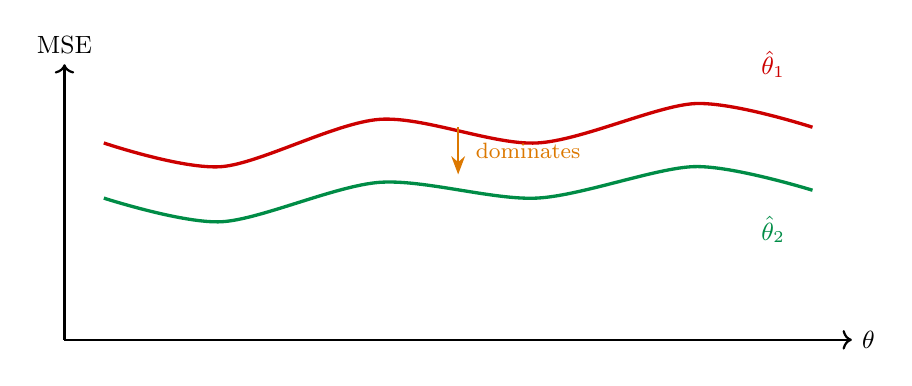
\begin{tikzpicture}
  \draw[thick, ->] (0, 0) -- (10, 0) node[right, font=\small] {$\theta$};
  \draw[thick, ->] (0, 0) -- (0, 3.5) node[above, font=\small] {MSE};

  % Estimator 1 (dominated)
  \draw[very thick, sampred, smooth] plot coordinates {
    (0.5, 2.5) (2, 2.2) (4, 2.8) (6, 2.5) (8, 3.0) (9.5, 2.7)
  };
  \node[font=\small\bfseries, sampred] at (9, 3.5) {$\hat\theta_1$};

  % Estimator 2 (dominates)
  \draw[very thick, paramgreen, smooth] plot coordinates {
    (0.5, 1.8) (2, 1.5) (4, 2.0) (6, 1.8) (8, 2.2) (9.5, 1.9)
  };
  \node[font=\small\bfseries, paramgreen] at (9, 1.4) {$\hat\theta_2$};

  % Arrow
  \draw[-{Stealth}, thick, orange1] (5, 2.7) -- (5, 2.1);
  \node[font=\footnotesize, orange1, right] at (5.1, 2.4) {dominates};
\end{tikzpicture}
\end{center}

\vspace{0.1cm}
\begin{center}
\small $\hat\theta_1$ is \textbf{inadmissible} --- $\hat\theta_2$ is at least as good everywhere, and strictly better somewhere.
\end{center}
\end{frame}

\begin{frame}
\frametitle{Stein's Paradox (1956)}

\vspace{-0.1cm}
\begin{center}
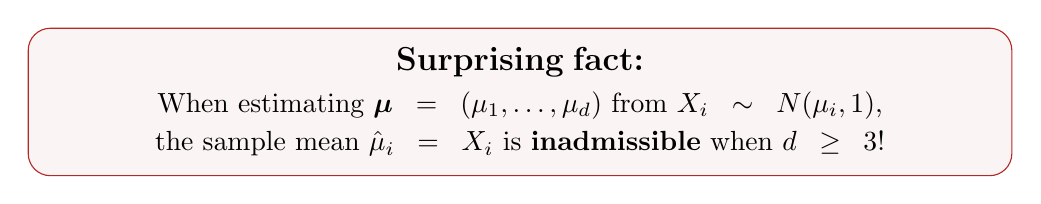
\begin{tikzpicture}
  \node[draw=warnred, fill=warnred!5, rounded corners=8pt, text width=12cm, align=center, inner sep=7pt] {
    {\large\bfseries Surprising fact:}\\[3pt]
    When estimating $\boldsymbol{\mu} = (\mu_1, \ldots, \mu_d)$ from $X_i \sim N(\mu_i, 1)$,\\[2pt]
    the sample mean $\hat\mu_i = X_i$ is \textbf{inadmissible} when $d \geq 3$!
  };
\end{tikzpicture}
\end{center}

\vspace{-0.05cm}
\begin{columns}[T]
\begin{column}{0.52\textwidth}
\small
The \textbf{James--Stein estimator} dominates it:
$$\hat\mu_i^{\,JS} = \left(1 - \frac{d-2}{\|\mathbf{X}\|^2}\right) X_i$$

\vspace{-0.25cm}
\begin{itemize}\setlength{\itemsep}{0pt}
  \small
  \item \textbf{Shrinks} each $X_i$ toward $0$
  \item Works even if $\mu_i$'s are unrelated!
  \item A little bias buys a lot of\\variance reduction
\end{itemize}
\end{column}
\begin{column}{0.46\textwidth}
\begin{center}
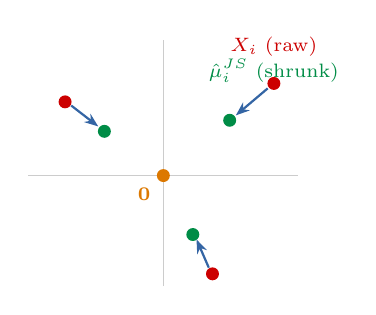
\begin{tikzpicture}[scale=0.78]
  % Axes
  \draw[gray!40, thin] (-2.2, 0) -- (2.2, 0);
  \draw[gray!40, thin] (0, -1.8) -- (0, 2.2);

  % Origin
  \fill[orange1] (0, 0) circle (3pt);
  \node[font=\scriptsize, orange1, below left] at (-0.05, -0.05) {$\mathbf{0}$};

  % Point 1
  \fill[sampred] (1.8, 1.5) circle (3pt);
  \fill[paramgreen] (1.08, 0.9) circle (3pt);
  \draw[-{Stealth[length=5pt]}, popblue, thick] (1.7, 1.42) -- (1.18, 0.98);

  % Point 2
  \fill[sampred] (-1.6, 1.2) circle (3pt);
  \fill[paramgreen] (-0.96, 0.72) circle (3pt);
  \draw[-{Stealth[length=5pt]}, popblue, thick] (-1.5, 1.14) -- (-1.06, 0.8);

  % Point 3
  \fill[sampred] (0.8, -1.6) circle (3pt);
  \fill[paramgreen] (0.48, -0.96) circle (3pt);
  \draw[-{Stealth[length=5pt]}, popblue, thick] (0.74, -1.5) -- (0.54, -1.04);

  % Legend
  \node[font=\scriptsize, sampred] at (1.8, 2.1) {$X_i$ (raw)};
  \node[font=\scriptsize, paramgreen] at (1.8, 1.7) {$\hat\mu_i^{JS}$ (shrunk)};
\end{tikzpicture}
\end{center}
\end{column}
\end{columns}

\vspace{-0.05cm}
\begin{center}
\small Paradox: estimating the average temperature in Yerevan \emph{improves} if you\\
jointly estimate it with the price of tea in China and the height of the Eiffel Tower.
\end{center}
\end{frame}

\begin{frame}
\frametitle{Minimax Estimators}

\small A \textbf{minimax} estimator minimizes the \textbf{worst-case} risk:
$$\hat\theta_{\text{minimax}} = \arg\min_{\hat\theta}\; \max_{\theta}\; \text{MSE}(\hat\theta, \theta)$$

\vspace{-0.2cm}
\begin{center}
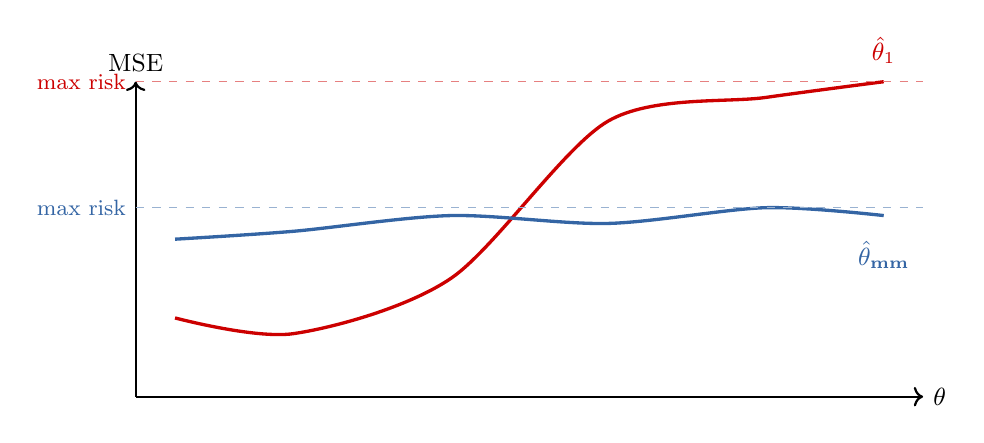
\begin{tikzpicture}
  \draw[thick, ->] (0, 0) -- (10, 0) node[right, font=\small] {$\theta$};
  \draw[thick, ->] (0, 0) -- (0, 4) node[above, font=\small] {MSE};

  % Estimator 1: high in some places
  \draw[very thick, sampred, smooth] plot coordinates {
    (0.5, 1.0) (2, 0.8) (4, 1.5) (6, 3.5) (8, 3.8) (9.5, 4.0)
  };
  \node[font=\small\bfseries, sampred] at (9.5, 4.4) {$\hat\theta_1$};
  \draw[dashed, sampred!50] (0, 4.0) -- (10, 4.0);
  \node[left, font=\footnotesize, sampred] at (0, 4.0) {max risk};

  % Minimax: flatter
  \draw[very thick, popblue, smooth] plot coordinates {
    (0.5, 2.0) (2, 2.1) (4, 2.3) (6, 2.2) (8, 2.4) (9.5, 2.3)
  };
  \node[font=\small\bfseries, popblue] at (9.5, 1.8) {$\hat\theta_{\text{mm}}$};
  \draw[dashed, popblue!50] (0, 2.4) -- (10, 2.4);
  \node[left, font=\footnotesize, popblue] at (0, 2.4) {max risk};
\end{tikzpicture}
\end{center}

\vspace{-0.1cm}
\begin{center}
\small Minimax = \textbf{conservative}: protects against the worst $\theta$. Minimax hedges.
\end{center}
\end{frame}

\begin{frame}
\frametitle{Three Philosophies of Estimation}
\begin{center}
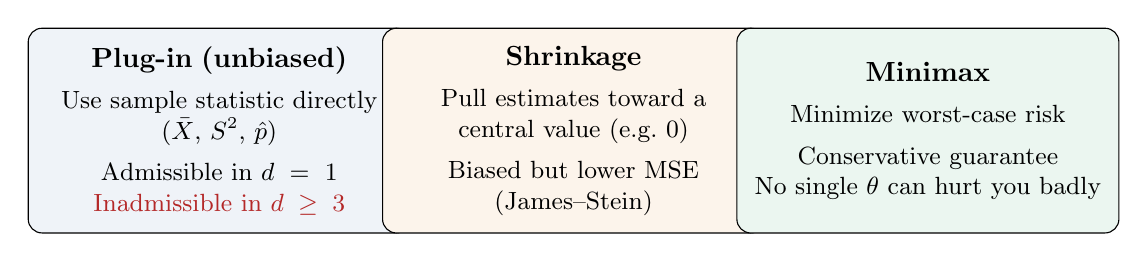
\begin{tikzpicture}[
  rbox/.style={draw, rounded corners=5pt, minimum width=4.8cm, minimum height=2.6cm, align=center, text width=4.5cm, inner sep=5pt, font=\small}
]
  \node[rbox, fill=popblue!8] at (-4.5, 0) {
    \textbf{\normalsize Plug-in (unbiased)}\\[4pt]
    Use sample statistic directly\\
    ($\bar{X}$, $S^2$, $\hat{p}$)\\[4pt]
    Admissible in $d = 1$\\
    \textcolor{warnred}{Inadmissible in $d \geq 3$}
  };
  \node[rbox, fill=orange1!8] at (0, 0) {
    \textbf{\normalsize Shrinkage}\\[4pt]
    Pull estimates toward a\\
    central value (e.g.\ $0$)\\[4pt]
    Biased but lower MSE\\
    (James--Stein)
  };
  \node[rbox, fill=paramgreen!8] at (4.5, 0) {
    \textbf{\normalsize Minimax}\\[4pt]
    Minimize worst-case risk\\[4pt]
    Conservative guarantee\\
    No single $\theta$ can hurt you badly
  };
\end{tikzpicture}
\end{center}

\vspace{0.2cm}
\begin{center}
\fcolorbox{violet1}{violet1!5}{\parbox{11cm}{\centering\small
  \textbf{Takeaway:} In high dimensions ($d \geq 3$), shrinkage estimators are provably better\\
  than using each sample statistic on its own. We'll see more of this in later lectures.
}}
\end{center}
\end{frame}

% ============================================================
\section{Summary}

\begin{frame}
\frametitle{Summary: How to Judge an Estimator}
\begin{center}
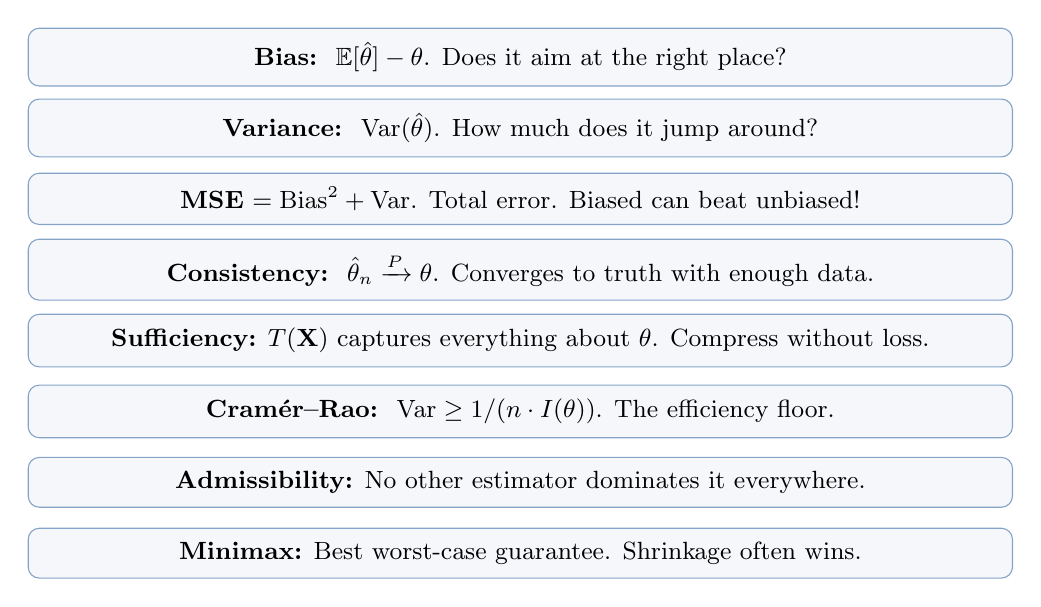
\begin{tikzpicture}[
  sbox/.style={draw=popblue!60, fill=popblue!5, rounded corners=4pt, minimum width=12.5cm, minimum height=0.6cm, align=left, inner sep=5pt, font=\small}
]
  \node[sbox] at (0, 3.15) {\textbf{Bias:} $\;\mathbb{E}[\hat\theta] - \theta$. Does it aim at the right place?};
  \node[sbox] at (0, 2.25) {\textbf{Variance:} $\;\text{Var}(\hat\theta)$. How much does it jump around?};
  \node[sbox] at (0, 1.35) {\textbf{MSE} $= \text{Bias}^2 + \text{Var}$. Total error. Biased can beat unbiased!};
  \node[sbox] at (0, 0.45) {\textbf{Consistency:} $\;\hat\theta_n \xrightarrow{P} \theta$. Converges to truth with enough data.};
  \node[sbox] at (0, -0.45) {\textbf{Sufficiency:} $T(\mathbf{X})$ captures everything about $\theta$. Compress without loss.};
  \node[sbox] at (0, -1.35) {\textbf{Cram\'er--Rao:} $\;\text{Var} \geq 1/(n \cdot I(\theta))$. The efficiency floor.};
  \node[sbox] at (0, -2.25) {\textbf{Admissibility:} No other estimator dominates it everywhere.};
  \node[sbox] at (0, -3.15) {\textbf{Minimax:} Best worst-case guarantee. Shrinkage often wins.};
\end{tikzpicture}
\end{center}
\end{frame}

\begin{frame}
\frametitle{Homework}
\begin{enumerate}
  \item Show that $\bar{X}$ is unbiased for $\mu$ and compute its MSE.

  \vspace{0.2cm}
  \item Show that $\hat\sigma^2_n = \frac{1}{n}\sum(X_i - \bar{X})^2$ is biased for $\sigma^2$. Find the bias.

  \vspace{0.2cm}
  \item Compute the Fisher information $I(\theta)$ for $\text{Poisson}(\lambda)$.\\
    Use it to find the Cram\'er--Rao lower bound for estimating $\lambda$.\\
    Is $\hat\lambda = \bar{X}$ efficient?

  \vspace{0.2cm}
  \item Suppose you shrink $\bar{X}$ toward 0: $\;\hat\mu_c = c\bar{X}$ for $0 < c < 1$.\\
    Find the bias, variance, and MSE as functions of $c$.\\
    For what value of $c$ is MSE minimized? Is the optimal estimator biased?

  \vspace{0.2cm}
  \item Use the factorization theorem to show that $T = \sum X_i$ is a sufficient statistic\\
    for $\lambda$ when $X_1, \ldots, X_n \sim \text{Poisson}(\lambda)$.
\end{enumerate}
\end{frame}

\begin{frame}
\begin{center}
  {\Huge\bfseries\textcolor{popblue}{Questions?}}
\end{center}
\end{frame}

\end{document}
